\section{Tuning module}

in Snowman this is translated to one filter of each type per rule per sensor.

If a filter occurs inline, this filter is regarded as a default filter and will
be active on every sensor where the rule operates. A user can choose to
override the default filter on a sensor by defining a custom filter to be used
on the respective sensor.


To stop \snort from adding duplicate filters, all inline filters
are removed from the rulestrings. Any filters extracted from
the rulestring are written as plain text (i.e. as they appear in the original
rulestring) in the \textit{filters} field of the rule revision object. This is
to ensure that all the original rule options are stored meaning that no data is
lost or discarded. 

 Filters are removed from the rulestring and
transformed into event filter and detection filter objects.

\begin{figure}
\centering
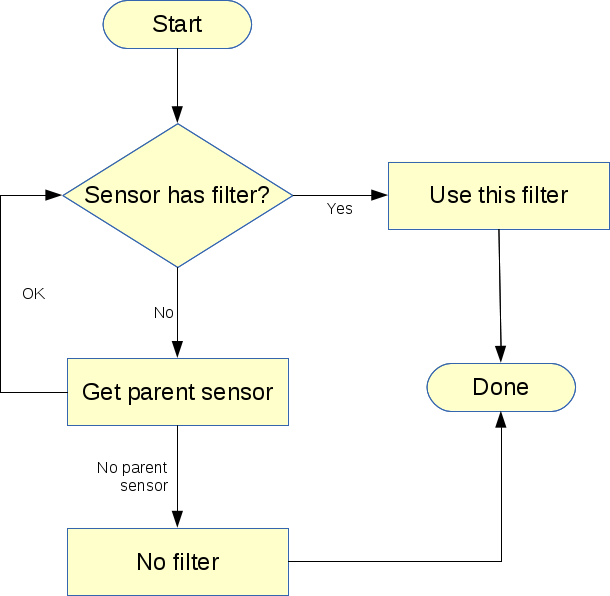
\includegraphics[scale=0.4]{./img/filter_flowchart.png}
\caption{Flow}
\label{fig:filter_flowchart}
\end{figure}